\chapter{Introducción}
\label{cap:intro}

Este manual acompaña al paquete de simulación \code{ball\_plate}, cuarto experimento de la serie de sistemas de control. Es la extensión a dos dimensiones de la bola y viga~\cite{viga}: conviene haber trabajado antes con ella, porque cada eje del plato se comporta, en primera aproximación, como una bola y viga. Está organizado en dos partes:
\begin{itemize}
  \item \textbf{Parte teórica} (capítulos~\ref{cap:modelo}--\ref{cap:control}): modelo dinámico, análisis lineal, la cámara como sensor y diseño de controladores.
  \item \textbf{Parte práctica} (capítulos~\ref{cap:simulink}--\ref{cap:practicas}): el modelo Simulink, la interfaz de código, la interfaz gráfica y una serie de prácticas guiadas.
\end{itemize}
Los resultados numéricos y todas las gráficas de este manual se han obtenido simulando el modelo Simulink del paquete (MATLAB R2025b) y se han contrastado con una réplica independiente en Python (apéndice~\ref{cap:validacion}).

\section{El sistema}

Una bola de acero rueda sobre un plato cuadrado de \SI{30}{cm} de lado. El plato está sujeto en su centro por una cardán de dos ejes~\cite{awtar2002} (figura~\ref{fig:sistema}):
\begin{itemize}
  \item el \textbf{motor A}, fijo a la base, gira el marco exterior un ángulo $\alpha$ alrededor del eje $y$;
  \item el \textbf{motor B}, montado sobre el marco exterior, gira el plato un ángulo $\beta$ alrededor del eje $x$.
\end{itemize}
Una \textbf{cámara cenital} ve el plato desde arriba y entrega la posición de la bola 50 veces por segundo, con un fotograma de retraso. Los dos ángulos del plato se miden con encoders. El objetivo es llevar la bola a un punto o hacerla seguir una trayectoria (una circunferencia, un ocho, un cuadrado).

\begin{figure}[H]
\centering
% Esquema de la bola y plato (perspectiva caballera simplificada)
\begin{tikzpicture}[>=Latex,font=\small,x={(1cm,0cm)},y={(0.55cm,0.38cm)},z={(0cm,1cm)}]
\def\a{3}
% base y poste
\fill[gray!15] (-4,-4,-2.6) -- (4,-4,-2.6) -- (4,4,-2.6) -- (-4,4,-2.6) -- cycle;
\fill[gray!45] (-0.2,0,-2.6) rectangle (0.2,0,-0.25);
% motor A (fijo, lado -y)
\fill[c1!30,draw=c1!60!black] (-0.35,-\a-0.9,-1.0) rectangle (0.35,-\a-0.9,-0.1);
\node[font=\scriptsize,c1!60!black,anchor=north] at (0,-\a-0.9,-1.05) {motor A ($\alpha$)};
\draw[c1!60!black,thick] (0,-\a-0.9,-0.4) -- (0,-\a-0.2,-0.4) -- (0,-\a-0.2,0);
% motor B (sobre el marco exterior, lado +x)
\fill[c2!30,draw=c2!60!black] (\a+0.6,-0.35,-0.8) -- (\a+0.6,0.35,-0.8) -- (\a+0.6,0.35,0) -- (\a+0.6,-0.35,0) -- cycle;
\node[font=\scriptsize,c2!60!black,anchor=west] at (\a+0.8,0,-0.6) {motor B ($\beta$)};
% marco exterior del cardán
\draw[gray!60!black,very thick] (-\a-0.3,-\a-0.3,0) -- (\a+0.3,-\a-0.3,0) -- (\a+0.3,\a+0.3,0) -- (-\a-0.3,\a+0.3,0) -- cycle;
% plato
\fill[c1!10,draw=c1!70!black,thick,opacity=0.9] (-\a,-\a,0) -- (\a,-\a,0) -- (\a,\a,0) -- (-\a,\a,0) -- cycle;
\foreach \v in {-2,-1,0,1,2} {
  \draw[c1!25] (\v,-\a,0) -- (\v,\a,0);
  \draw[c1!25] (-\a,\v,0) -- (\a,\v,0);
}
% ejes
\draw[->,c4,thick] (0,0,0) -- (\a+0.9,0,0) node[right]{$x$};
\draw[->,c4,thick] (0,0,0) -- (0,\a+1.2,0) node[above]{$y$};
\draw[->,gray] (0,0,0) -- (0,0,1.9) node[above]{$z$};
% bola
\node[circle,shading=ball,ball color=gray!55,minimum size=0.55cm,inner sep=0pt] at (1.6,1.1,0.28) {};
\draw[c4,densely dotted] (1.6,0,0) -- (1.6,1.1,0) -- (0,1.1,0);
\node[c4,font=\scriptsize,below] at (1.6,0,0) {$x$};
\node[c4,font=\scriptsize,left] at (0,1.1,0) {$y$};
% giros
\draw[->,thick,c1!70!black] (-0.6,-\a-0.6,0.5) arc[start angle=150,end angle=30,radius=0.7];
\node[c1!70!black] at (0,-\a-0.6,1.15) {$\alpha$};
\draw[->,thick,c2!70!black] (\a+0.5,0.6,0.5) arc[start angle=150,end angle=30,radius=0.6];
\node[c2!70!black] at (\a+0.6,0,1.1) {$\beta$};
% cámara
\fill[gray!70] (-0.3,0,3.0) rectangle (0.3,0,3.4);
\draw[gray,dashed] (-0.3,0,3.0) -- (-\a,-\a,0.05);
\draw[gray,dashed] (0.3,0,3.0) -- (\a,\a,0.05);
\node[font=\scriptsize,anchor=west] at (0.4,0,3.2) {cámara cenital (50 fps)};
\end{tikzpicture}

\caption{Bola y plato. El motor A inclina el plato un ángulo $\alpha$ (alrededor de $y$, mueve la bola en $x$); el motor B, que viaja con el marco exterior, lo inclina un ángulo $\beta$ (alrededor de $x$, mueve la bola en $y$).}
\label{fig:sistema}
\end{figure}

Frente a la bola y viga hay tres novedades:
\begin{enumerate}
  \item \textbf{Dos entradas y dos salidas}. Cerca del centro y con el plato horizontal los dos ejes se desacoplan, y se puede diseñar un controlador por eje. Lejos del centro o con movimientos rápidos aparecen acoplamientos no lineales, y se puede medir cuánto importan.
  \item \textbf{La cámara es un sensor lento y con retraso}: \SI{50}{Hz} frente a los \SI{500}{Hz} del controlador, y un fotograma (\SI{20}{ms}) de latencia. Es la principal limitación de este experimento, y obliga a trabajar con un sistema multifrecuencia.
  \item \textbf{Las referencias son trayectorias planas}, lo que permite estudiar el seguimiento de una forma más visual que con una referencia escalar.
\end{enumerate}

\begin{table}[H]
\centering\small
\begin{tabular}{@{}lll@{}}
\toprule
Símbolo & Significado & Convenio\\
\midrule
$x$, $y$ & posición de la bola [m] & $0$ = centro del plato; borde en $\pm\SI{13.7}{cm}$ en cada eje\\
$\alpha$ & inclinación alrededor de $y$ [rad] & $\alpha>0$ \textbf{levanta} el borde $+x$ (la bola rueda hacia $-x$); motor A\\
$\beta$ & inclinación alrededor de $x$ [rad] & $\beta>0$ \textbf{levanta} el borde $+y$ (la bola rueda hacia $-y$); motor B\\
$V_a$, $V_b$ & tensiones de los motores [V] & saturación $\pm\SI{10}{V}$; topes de inclinación en $\pm15^\circ$\\
$\vect s$ & estado & $[x,\ \xd,\ y,\ \yd,\ \alpha,\ \ald,\ \beta,\ \bed]^\top$\\
\bottomrule
\end{tabular}
\caption{Variables y convenio de signos.}
\label{tab:convenio}
\end{table}

\begin{nota}
La interfaz de código trabaja en \textbf{metros y radianes}. La interfaz gráfica y los campos \code{*\_cm} y \code{*\_deg} de los resultados (\code{x\_cm}, \code{y\_cm}, \code{rx\_cm}, \code{ry\_cm}, \code{al\_deg}, \code{be\_deg}) usan centímetros y grados.
\end{nota}

\section{Contenido del paquete}

\begin{table}[H]
\centering\small
\begin{tabularx}{\linewidth}{@{}lX@{}}
\toprule
Archivo & Contenido\\
\midrule
\code{bp\_params.m} & Parámetros físicos, de los motores, de la cámara y de los controladores.\\
\code{bp\_derived.m}, \code{bp\_linearize.m}, \code{bp\_lqr.m}, \code{bp\_design.m} & Magnitudes derivadas, linealización por eje, LQR (con o sin toolbox) y cálculo de ganancias.\\
\code{bp\_plant\_block.m} & Dinámica no lineal de 4 grados de libertad con dos motores (código del bloque de la planta).\\
\code{bp\_controller\_block.m} & Controlador discreto multifrecuencia con 4 modos.\\
\code{bp\_ref\_block.m} & Generador de trayectorias: punto, circunferencia, cuadrado, ocho o externa.\\
\code{bp\_build\_model.m} & Genera el modelo \code{ballplate\_sim.slx} mediante un script.\\
\code{BallPlate.m} & Clase con la interfaz de código: ensayos por lotes y control en vivo.\\
\code{bp\_gui.m} & Interfaz gráfica en vivo con animación 3D y vista de la cámara.\\
\code{bp\_draw.m}, \code{bp\_draw\_top.m}, \code{bp\_view.m}, \code{bp\_animate.m}, \code{bp\_plot\_results.m} & Escena 3D, vista cenital, puntos de vista, reproducción de ensayos y gráficas.\\
\code{examples.m} & Recorrido guiado por secciones.\\
\code{python\_reference\_sim.py} & Réplica independiente en Python usada para validar el modelo.\\
\code{validation/} & Scripts de validación cruzada Simulink--Python (apéndice~\ref{cap:validacion}).\\
\bottomrule
\end{tabularx}
\caption{Archivos del paquete \code{ball\_plate}.}
\label{tab:archivos}
\end{table}

\section{Requisitos y puesta en marcha}

Se necesita MATLAB y Simulink R2020b o posterior (se ha probado con R2025b). La Control System Toolbox es opcional: si no está instalada, \code{bp\_lqr} resuelve la ecuación de Riccati por el método del Hamiltoniano.

\begin{lstlisting}[caption={Primeros pasos.}]
cd src/ball_plate
bp_build_model                 % crea ballplate_sim.slx (solo la primera vez)
bp_gui                         % interfaz gráfica en vivo
% o desde código:
bp = BallPlate();
bp.setMode('lqr');
bp.setRef('circle', [0 0], 0.06, 0.2);   % circunferencia de 6 cm a 0,2 Hz
res = bp.run(15);
bp_plot_results(res); bp.animate(res);
\end{lstlisting}

\begin{figure}[H]
\centering
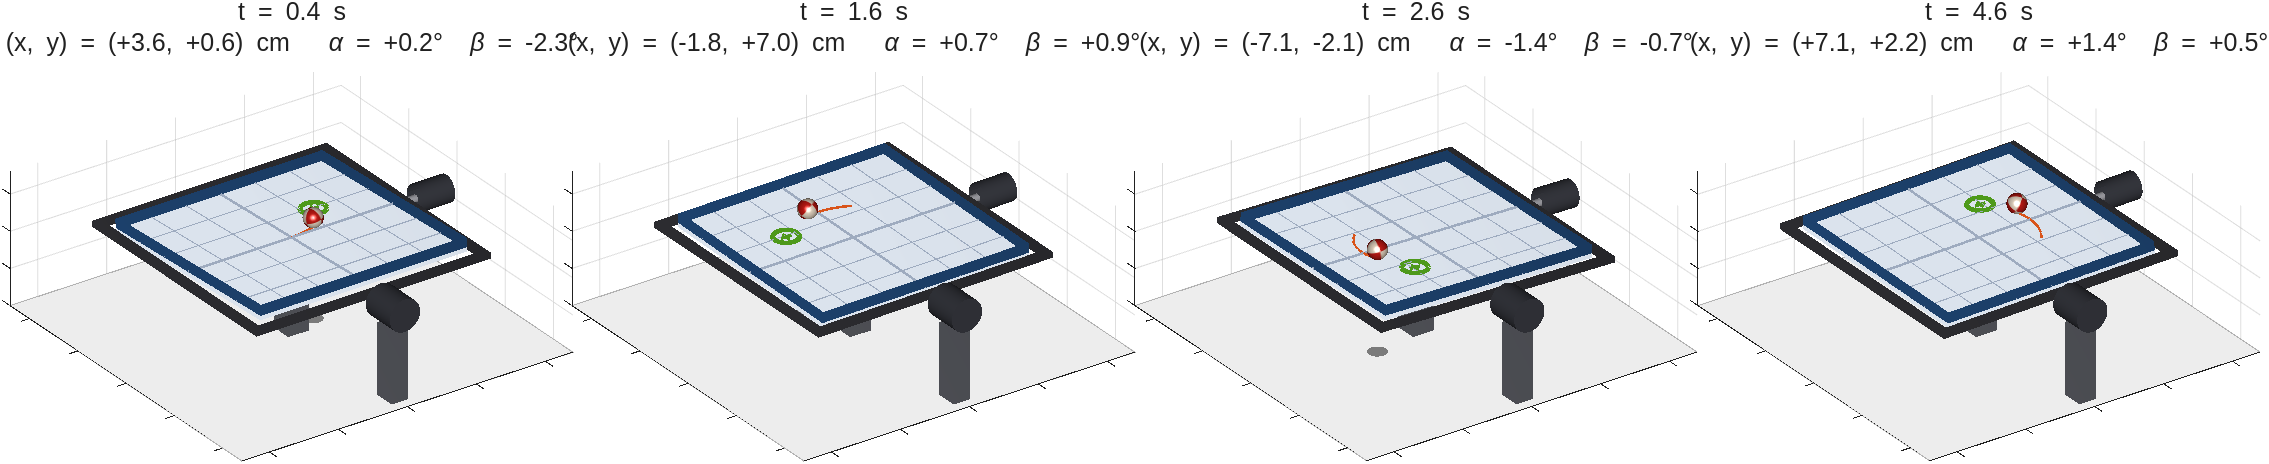
\includegraphics[width=\linewidth]{data/frames.png}
\caption{Fotogramas de la animación 3D (\code{bp\_animate}) siguiendo una circunferencia de \SI{8}{cm} a \SI{0.25}{Hz} con el LQR. La estela naranja muestra el último tramo recorrido y el anillo verde la referencia.}
\label{fig:frames}
\end{figure}
